\subsection{Nearest Neighbor Classifier}
	\textbf{Student Name: }Christian Stevandy \textbf{ID:} 0870945\\\\
	This section describes training classifier with nearest neighbors and integration with other classifiers.
\subsubsection*{Motivation}
	Classified posts help users to navigate the posts they are interested in and NN classifier is one simple effective way to classify documents. Our project generates model using multiple classifiers, so it is required to integrate all the classifier we used which are NN, Support Vector Machine and Naïve Bayes in one result with ensemble learning.
\subsubsection*{Problem formulation}
	Given a collection of user posts and training set. This task train classifier, classify post with its topic and define the final label for all post with ensemble learning.
\subsubsection*{Approach}
	We created this classifier using nearest neighbor in Weka. Ensemble learning is implemented by majority vote.\\\\
	\textbf{a. Nearest Neighbor} \\
		Nearest Neighbor is a simple classifier defines class by finding nearest distances of its instance. User post is represented as a collection of word in a vector space model and in vector space model, it is possible to measure distance by Euclidean Distance .This classifier based on Instance-based learning algorithms D, Aha, D.Kibler (1991): \\
	\begin{figure}[h]
		\begin{center}
			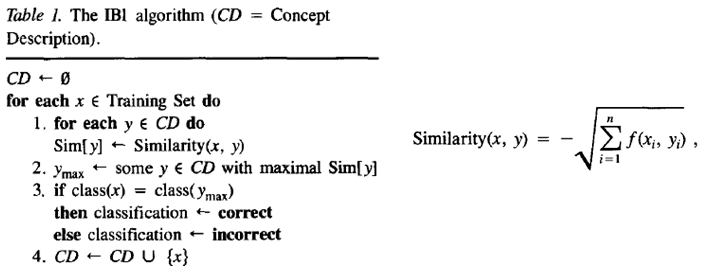
\includegraphics[scale=0.8]{images/NN1.png}
		\caption{Post Index\label{NN1}}
		\end{center}
	\end{figure}
		With the algorithm in \ref{NN1} we can find similarity which are the nearest distance between between each instance and classify based on the distance. The similarity in this algorithm is a Euclidean distance.\\\\
	\textbf{b. Simple Vote Ensemble Learning} \\
		Ensemble learning is used to combine every classifier we used in this project. Ensemble learning that implemented in this task are based on Leo Breiman (1996). Bagging predictors. Machine Learning. 24(2):123-140		 \\\\Our Ensemble Learning is using a simple majority vote for every trained instance.\\\\
		Algorithm:\\
		   1. Classify post using prediction = NN, Support Vector Machine, Naïve Bayes.\\
		   2. Final prediction = majority prediction.\\
		   3. If no majority randomize the prediction.\\\\
	\textbf{c. Implementation} \\
	\begin{figure}[h]
		\begin{center}
			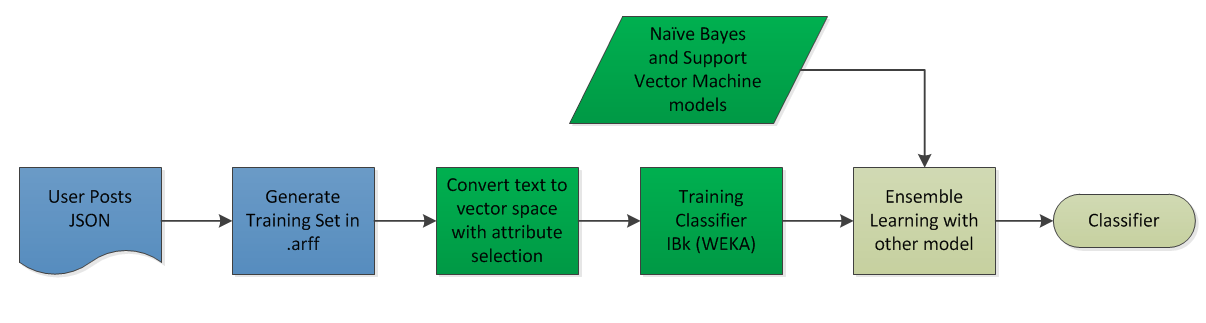
\includegraphics[scale=0.45]{images/Nearest.png}
		\caption{Post Index\label{Nearest}}
		\end{center}
	\end{figure}
	\\Labeled user posts are used in training set. In order for Weka to use the user posts that are generated from crawler, json file that consist of user posts is converted to .arff. And then it is used for trains classifier. After the nearest neighbor classifier is trained, it generates model that will be used along with other classifier models to classify a post in an ensemble learning.\
\subsubsection*{Evaluation}
	The training set data can be used for training and evaluating a classifier using cross-validation. The evaluation for ensemble learning is done manually.\\\\
	Result of 10 folds cross-validation using one sample training set:\\\\\\\\\\\\\\\
\begin{table}
\centering
    \begin{tabular}{|l|l|} \hline
    Correctly Classified Instances   & 1120(87.5684 \%) \\ \hline
    Incorrectly Classified Instances & 159(12.4316 \%)  \\ \hline
    Kappa statistic                  & 0.7987          \\ \hline
    Mean absolute error              & 0.0869          \\ \hline
    Root mean squared error          & 0.268           \\ \hline
    Relative absolute error          & 21.04\%          \\ \hline
    Root relative squared error      & 58.98\%s          \\ \hline
    Total Number of Instances        & 1279            \\ \hline
    \end{tabular}
	\caption{Nearest Neighbor Evaluation\label{nn_table}}
\end{table}
	\\From the table~\ref{nn_table} of cross-validation and manual evaluation the classifier is good to be used.\\

	
	
	